% Options for packages loaded elsewhere
\PassOptionsToPackage{unicode}{hyperref}
\PassOptionsToPackage{hyphens}{url}
\PassOptionsToPackage{dvipsnames,svgnames,x11names}{xcolor}
%
\documentclass[
  letterpaper,
  DIV=11,
  numbers=noendperiod]{scrartcl}

\usepackage{amsmath,amssymb}
\usepackage{iftex}
\ifPDFTeX
  \usepackage[T1]{fontenc}
  \usepackage[utf8]{inputenc}
  \usepackage{textcomp} % provide euro and other symbols
\else % if luatex or xetex
  \usepackage{unicode-math}
  \defaultfontfeatures{Scale=MatchLowercase}
  \defaultfontfeatures[\rmfamily]{Ligatures=TeX,Scale=1}
\fi
\usepackage{lmodern}
\ifPDFTeX\else  
    % xetex/luatex font selection
\fi
% Use upquote if available, for straight quotes in verbatim environments
\IfFileExists{upquote.sty}{\usepackage{upquote}}{}
\IfFileExists{microtype.sty}{% use microtype if available
  \usepackage[]{microtype}
  \UseMicrotypeSet[protrusion]{basicmath} % disable protrusion for tt fonts
}{}
\makeatletter
\@ifundefined{KOMAClassName}{% if non-KOMA class
  \IfFileExists{parskip.sty}{%
    \usepackage{parskip}
  }{% else
    \setlength{\parindent}{0pt}
    \setlength{\parskip}{6pt plus 2pt minus 1pt}}
}{% if KOMA class
  \KOMAoptions{parskip=half}}
\makeatother
\usepackage{xcolor}
\setlength{\emergencystretch}{3em} % prevent overfull lines
\setcounter{secnumdepth}{-\maxdimen} % remove section numbering
% Make \paragraph and \subparagraph free-standing
\ifx\paragraph\undefined\else
  \let\oldparagraph\paragraph
  \renewcommand{\paragraph}[1]{\oldparagraph{#1}\mbox{}}
\fi
\ifx\subparagraph\undefined\else
  \let\oldsubparagraph\subparagraph
  \renewcommand{\subparagraph}[1]{\oldsubparagraph{#1}\mbox{}}
\fi

\usepackage{color}
\usepackage{fancyvrb}
\newcommand{\VerbBar}{|}
\newcommand{\VERB}{\Verb[commandchars=\\\{\}]}
\DefineVerbatimEnvironment{Highlighting}{Verbatim}{commandchars=\\\{\}}
% Add ',fontsize=\small' for more characters per line
\usepackage{framed}
\definecolor{shadecolor}{RGB}{241,243,245}
\newenvironment{Shaded}{\begin{snugshade}}{\end{snugshade}}
\newcommand{\AlertTok}[1]{\textcolor[rgb]{0.68,0.00,0.00}{#1}}
\newcommand{\AnnotationTok}[1]{\textcolor[rgb]{0.37,0.37,0.37}{#1}}
\newcommand{\AttributeTok}[1]{\textcolor[rgb]{0.40,0.45,0.13}{#1}}
\newcommand{\BaseNTok}[1]{\textcolor[rgb]{0.68,0.00,0.00}{#1}}
\newcommand{\BuiltInTok}[1]{\textcolor[rgb]{0.00,0.23,0.31}{#1}}
\newcommand{\CharTok}[1]{\textcolor[rgb]{0.13,0.47,0.30}{#1}}
\newcommand{\CommentTok}[1]{\textcolor[rgb]{0.37,0.37,0.37}{#1}}
\newcommand{\CommentVarTok}[1]{\textcolor[rgb]{0.37,0.37,0.37}{\textit{#1}}}
\newcommand{\ConstantTok}[1]{\textcolor[rgb]{0.56,0.35,0.01}{#1}}
\newcommand{\ControlFlowTok}[1]{\textcolor[rgb]{0.00,0.23,0.31}{#1}}
\newcommand{\DataTypeTok}[1]{\textcolor[rgb]{0.68,0.00,0.00}{#1}}
\newcommand{\DecValTok}[1]{\textcolor[rgb]{0.68,0.00,0.00}{#1}}
\newcommand{\DocumentationTok}[1]{\textcolor[rgb]{0.37,0.37,0.37}{\textit{#1}}}
\newcommand{\ErrorTok}[1]{\textcolor[rgb]{0.68,0.00,0.00}{#1}}
\newcommand{\ExtensionTok}[1]{\textcolor[rgb]{0.00,0.23,0.31}{#1}}
\newcommand{\FloatTok}[1]{\textcolor[rgb]{0.68,0.00,0.00}{#1}}
\newcommand{\FunctionTok}[1]{\textcolor[rgb]{0.28,0.35,0.67}{#1}}
\newcommand{\ImportTok}[1]{\textcolor[rgb]{0.00,0.46,0.62}{#1}}
\newcommand{\InformationTok}[1]{\textcolor[rgb]{0.37,0.37,0.37}{#1}}
\newcommand{\KeywordTok}[1]{\textcolor[rgb]{0.00,0.23,0.31}{#1}}
\newcommand{\NormalTok}[1]{\textcolor[rgb]{0.00,0.23,0.31}{#1}}
\newcommand{\OperatorTok}[1]{\textcolor[rgb]{0.37,0.37,0.37}{#1}}
\newcommand{\OtherTok}[1]{\textcolor[rgb]{0.00,0.23,0.31}{#1}}
\newcommand{\PreprocessorTok}[1]{\textcolor[rgb]{0.68,0.00,0.00}{#1}}
\newcommand{\RegionMarkerTok}[1]{\textcolor[rgb]{0.00,0.23,0.31}{#1}}
\newcommand{\SpecialCharTok}[1]{\textcolor[rgb]{0.37,0.37,0.37}{#1}}
\newcommand{\SpecialStringTok}[1]{\textcolor[rgb]{0.13,0.47,0.30}{#1}}
\newcommand{\StringTok}[1]{\textcolor[rgb]{0.13,0.47,0.30}{#1}}
\newcommand{\VariableTok}[1]{\textcolor[rgb]{0.07,0.07,0.07}{#1}}
\newcommand{\VerbatimStringTok}[1]{\textcolor[rgb]{0.13,0.47,0.30}{#1}}
\newcommand{\WarningTok}[1]{\textcolor[rgb]{0.37,0.37,0.37}{\textit{#1}}}

\providecommand{\tightlist}{%
  \setlength{\itemsep}{0pt}\setlength{\parskip}{0pt}}\usepackage{longtable,booktabs,array}
\usepackage{calc} % for calculating minipage widths
% Correct order of tables after \paragraph or \subparagraph
\usepackage{etoolbox}
\makeatletter
\patchcmd\longtable{\par}{\if@noskipsec\mbox{}\fi\par}{}{}
\makeatother
% Allow footnotes in longtable head/foot
\IfFileExists{footnotehyper.sty}{\usepackage{footnotehyper}}{\usepackage{footnote}}
\makesavenoteenv{longtable}
\usepackage{graphicx}
\makeatletter
\def\maxwidth{\ifdim\Gin@nat@width>\linewidth\linewidth\else\Gin@nat@width\fi}
\def\maxheight{\ifdim\Gin@nat@height>\textheight\textheight\else\Gin@nat@height\fi}
\makeatother
% Scale images if necessary, so that they will not overflow the page
% margins by default, and it is still possible to overwrite the defaults
% using explicit options in \includegraphics[width, height, ...]{}
\setkeys{Gin}{width=\maxwidth,height=\maxheight,keepaspectratio}
% Set default figure placement to htbp
\makeatletter
\def\fps@figure{htbp}
\makeatother

\KOMAoption{captions}{tableheading}
\makeatletter
\@ifpackageloaded{caption}{}{\usepackage{caption}}
\AtBeginDocument{%
\ifdefined\contentsname
  \renewcommand*\contentsname{Table of contents}
\else
  \newcommand\contentsname{Table of contents}
\fi
\ifdefined\listfigurename
  \renewcommand*\listfigurename{List of Figures}
\else
  \newcommand\listfigurename{List of Figures}
\fi
\ifdefined\listtablename
  \renewcommand*\listtablename{List of Tables}
\else
  \newcommand\listtablename{List of Tables}
\fi
\ifdefined\figurename
  \renewcommand*\figurename{Figure}
\else
  \newcommand\figurename{Figure}
\fi
\ifdefined\tablename
  \renewcommand*\tablename{Table}
\else
  \newcommand\tablename{Table}
\fi
}
\@ifpackageloaded{float}{}{\usepackage{float}}
\floatstyle{ruled}
\@ifundefined{c@chapter}{\newfloat{codelisting}{h}{lop}}{\newfloat{codelisting}{h}{lop}[chapter]}
\floatname{codelisting}{Listing}
\newcommand*\listoflistings{\listof{codelisting}{List of Listings}}
\makeatother
\makeatletter
\makeatother
\makeatletter
\@ifpackageloaded{caption}{}{\usepackage{caption}}
\@ifpackageloaded{subcaption}{}{\usepackage{subcaption}}
\makeatother
\ifLuaTeX
  \usepackage{selnolig}  % disable illegal ligatures
\fi
\usepackage{bookmark}

\IfFileExists{xurl.sty}{\usepackage{xurl}}{} % add URL line breaks if available
\urlstyle{same} % disable monospaced font for URLs
\hypersetup{
  pdftitle={Homework 4},
  pdfauthor={Kevin Linares and Jamila Sani},
  colorlinks=true,
  linkcolor={blue},
  filecolor={Maroon},
  citecolor={Blue},
  urlcolor={Blue},
  pdfcreator={LaTeX via pandoc}}

\title{Homework 4}
\author{Kevin Linares and Jamila Sani}
\date{2024-09-29}

\begin{document}
\maketitle

\begin{center}\rule{0.5\linewidth}{0.5pt}\end{center}

\begin{Shaded}
\begin{Highlighting}[]
\ControlFlowTok{if}\NormalTok{ (}\SpecialCharTok{!}\FunctionTok{require}\NormalTok{(viridis)) }\FunctionTok{install.packages}\NormalTok{(}\StringTok{"viridis"}\NormalTok{, }\AttributeTok{repos =} \StringTok{"http://cran.us.r{-}project.org"}\NormalTok{)}
\end{Highlighting}
\end{Shaded}

\begin{verbatim}
Loading required package: viridis
\end{verbatim}

\begin{verbatim}
Loading required package: viridisLite
\end{verbatim}

\begin{Shaded}
\begin{Highlighting}[]
\ControlFlowTok{if}\NormalTok{ (}\SpecialCharTok{!}\FunctionTok{require}\NormalTok{(ggthemes)) }\FunctionTok{install.packages}\NormalTok{(}\StringTok{"ggthemes"}\NormalTok{, }\AttributeTok{repos =} \StringTok{"http://cran.us.r{-}project.org"}\NormalTok{)}
\end{Highlighting}
\end{Shaded}

\begin{verbatim}
Loading required package: ggthemes
\end{verbatim}

\begin{Shaded}
\begin{Highlighting}[]
\ControlFlowTok{if}\NormalTok{ (}\SpecialCharTok{!}\FunctionTok{require}\NormalTok{(broom)) }\FunctionTok{install.packages}\NormalTok{(}\StringTok{"broom"}\NormalTok{, }\AttributeTok{repos =} \StringTok{"http://cran.us.r{-}project.org"}\NormalTok{)}
\end{Highlighting}
\end{Shaded}

\begin{verbatim}
Loading required package: broom
\end{verbatim}

\begin{Shaded}
\begin{Highlighting}[]
\FunctionTok{require}\NormalTok{(ISLR2)}
\end{Highlighting}
\end{Shaded}

\begin{verbatim}
Loading required package: ISLR2
\end{verbatim}

\begin{Shaded}
\begin{Highlighting}[]
\FunctionTok{library}\NormalTok{(knitr)}
\FunctionTok{library}\NormalTok{(tidyverse)}
\end{Highlighting}
\end{Shaded}

\begin{verbatim}
-- Attaching core tidyverse packages ------------------------ tidyverse 2.0.0 --
v dplyr     1.1.4     v readr     2.1.5
v forcats   1.0.0     v stringr   1.5.1
v ggplot2   3.5.1     v tibble    3.2.1
v lubridate 1.9.3     v tidyr     1.3.1
v purrr     1.0.2     
\end{verbatim}

\begin{verbatim}
-- Conflicts ------------------------------------------ tidyverse_conflicts() --
x dplyr::filter() masks stats::filter()
x dplyr::lag()    masks stats::lag()
i Use the conflicted package (<http://conflicted.r-lib.org/>) to force all conflicts to become errors
\end{verbatim}

\begin{Shaded}
\begin{Highlighting}[]
\FunctionTok{data}\NormalTok{(Boston)}

\CommentTok{\# set a standard graphic theme for plots from the ggthemes package}
\FunctionTok{theme\_set}\NormalTok{(}\FunctionTok{theme\_hc}\NormalTok{())}

\NormalTok{print\_output }\OtherTok{\textless{}{-}} \ControlFlowTok{function}\NormalTok{(output, }\AttributeTok{cex =} \FloatTok{0.8}\NormalTok{) \{}
\NormalTok{  tmp }\OtherTok{\textless{}{-}} \FunctionTok{capture.output}\NormalTok{(output)}
  \FunctionTok{plot.new}\NormalTok{()}
  \FunctionTok{text}\NormalTok{(}\DecValTok{0}\NormalTok{, }\DecValTok{1}\NormalTok{, }\FunctionTok{paste}\NormalTok{(tmp, }\AttributeTok{collapse=}\StringTok{\textquotesingle{}}\SpecialCharTok{\textbackslash{}n}\StringTok{\textquotesingle{}}\NormalTok{), }\AttributeTok{adj =} \FunctionTok{c}\NormalTok{(}\DecValTok{0}\NormalTok{,}\DecValTok{1}\NormalTok{), }\AttributeTok{family =} \StringTok{\textquotesingle{}mono\textquotesingle{}}\NormalTok{, }\AttributeTok{cex =}\NormalTok{ cex)}
  \FunctionTok{box}\NormalTok{()}
\NormalTok{\}}

\CommentTok{\#options(scipen=999)}
\end{Highlighting}
\end{Shaded}

This exercise involves the Boston housing data set in ISLR2. Assume that
we are interested in median home values, medv.

\begin{enumerate}
\def\labelenumi{\arabic{enumi}.}
\tightlist
\item
  Examine medv as a function of crim, zn and indus in a multiple linear
  regres- sion.
\end{enumerate}

\subsection{A) Identify the predictors which are ``statistically
significant'' at α =
0.05.}\label{a-identify-the-predictors-which-are-statistically-significant-at-ux3b1-0.05.}

\begin{itemize}
\tightlist
\item
  All three predictors (crime rate per capita, proportion of residential
  land zoned for lots of 25k sq ft, and proportion of non-retail
  business acres per town) had a p-value of less than .05; therefore, we
  reject the null hypothesis that these variables are statistically
  different from 0.
\end{itemize}

\begin{Shaded}
\begin{Highlighting}[]
\CommentTok{\# set up pipeline from data to model results for linear models}
\NormalTok{m\_medv }\OtherTok{\textless{}{-}} \FunctionTok{lm}\NormalTok{(medv }\SpecialCharTok{\textasciitilde{}}\NormalTok{ crim }\SpecialCharTok{+}\NormalTok{ zn }\SpecialCharTok{+}\NormalTok{ indus, }\AttributeTok{data =}\NormalTok{ Boston)}

\FunctionTok{print\_output}\NormalTok{(}\FunctionTok{summary}\NormalTok{(m\_medv))}
\end{Highlighting}
\end{Shaded}

\begin{verbatim}
Warning in text.default(0, 1, paste(tmp, collapse = "\n"), adj = c(0, 1), :
font width unknown for character 0x09 in encoding latin1
\end{verbatim}

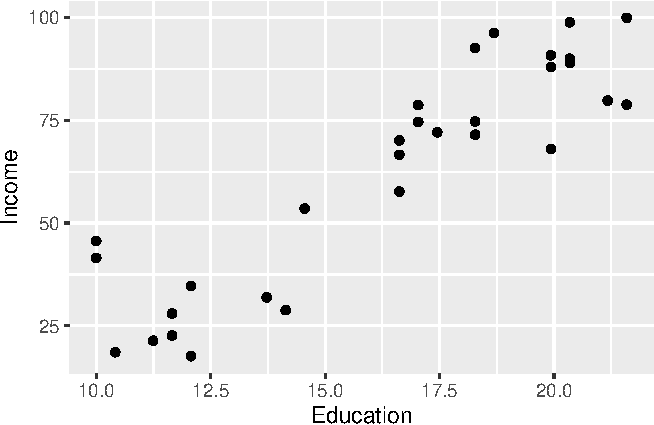
\includegraphics{HW4_files/figure-pdf/unnamed-chunk-2-1.pdf}

\subsection{B) List the null and alternative hypotheses tested in 1A and
your
conclusions.}\label{b-list-the-null-and-alternative-hypotheses-tested-in-1a-and-your-conclusions.}

\begin{itemize}
\tightlist
\item
  For multiple parameters, \(\beta\), the null we are testing in model
  1A is:
\end{itemize}

\[
H_0 : \beta_1 = \beta_2 = ... \beta_p = 0, \space \\
and \space each \space \beta_p = 0 
\]

\begin{itemize}
\item
  meaning that our null hypothesis is that each \(\beta\) coefficient is
  equal to each other and to \(0\).
\item
  Our alternative hypothesis: is that at least one of the three
  \(\beta\) coefficients are not equal to \(0\).
\item
  We reject the null hypothesis, and there is a useful linear
  relationship between median home value and one of the three predictors
  in the model.
\end{itemize}

\[
H_a : \beta_i \ne 0 \space (i = 1,...,p)
\]

\subsection{C) Interpret each of the regression coefficients as if it
were the primary exposure of
interest.}\label{c-interpret-each-of-the-regression-coefficients-as-if-it-were-the-primary-exposure-of-interest.}

\begin{itemize}
\item
  Do they make sense?
\item
  \(\beta_0\): When crime rate, the proportion of residential land zone,
  and the proportion of non-retail business acres all equal \(0\), the
  expected average income is \(\$27,395\) USD.
\item
  In this case, the intercept without centering predictors makes sense
  since there can be a suburb with 0 crime rate or 0 proportions.
\item
  \(\beta_{crim}\): For every additional crime rate per capita, we
  expect the median home value to drop \(.25\) or \(\$250\) USD, while
  holding other predictors variables constant.
\item
  \(\beta_{zn}\): For every one unit change in the proportion of
  residential land zoned for lots over 25,000 sq.ft., we expect the
  median home value to increase by \(.06\) or \(\$60\) USD, while
  holding other predictor variables constant.
\item
  \(\beta_{indus}\): For every one unit increase in the proportion of
  non-retail business acres per town, we expect the median home value to
  drop \(.42\) or \(\$420\) USD, while holding other predictor variables
  constant.
\end{itemize}

\subsection{D) It's generally not good practice to interpret all
predictors as if they were the exposure of
interest.}\label{d-its-generally-not-good-practice-to-interpret-all-predictors-as-if-they-were-the-exposure-of-interest.}

\begin{itemize}
\item
  Why do you think doing so could be problematic?
\item
  When creating these models the researcher typically has a hypothesis
  in mind guided by previous research and theory. Therefore, if we
  report every explanatory variable included in the model, we run the
  risk of capitalizing on spurious correlations, when two variables
  appear to be related by they are not (they are through a confounding
  variable). Furthermore, interpreting all predictors could be
  problematic because of the complexity of interpretation and making
  inferences. Also, multicollinearity and confounding issues may mask
  individual effects of each predictor.
\end{itemize}

\subsection{E) Construct and interpret 95\% confidence
intervals}\label{e-construct-and-interpret-95-confidence-intervals}

\begin{itemize}
\item
  For \(\hat{\beta_{crim}}\), \(\hat{\beta_{zn}}\), and
  \(\hat{\beta_{inuds}}\). (you do not need to calculate them ``by
  hand'').
\item
  How does the confidence intervals correspond to the hypotheses tested
  in 1A and 1B?
\item
  From the graphic we can quickly see whether any of the predictor's
  95\% confidence intervals capture 0, denoted by the blue line, which
  we do not observe to be the case for any of the predictors and we
  continue to reject the Null hypothesis \(\beta_p=0\).
\item
  If we were to draw 100 samples with size \(n\) from the same target
  population, we would expect 95\% of these samples to contain the true
  value of our \(\beta\) coefficients.
\end{itemize}

\begin{Shaded}
\begin{Highlighting}[]
\FunctionTok{confint}\NormalTok{(m\_medv, }\AttributeTok{level=}\NormalTok{.}\DecValTok{95}\NormalTok{) }
\end{Highlighting}
\end{Shaded}

\begin{verbatim}
                 2.5 %      97.5 %
(Intercept) 25.6954863 29.09380729
crim        -0.3348958 -0.16236084
zn           0.0241252  0.09287644
indus       -0.5408945 -0.29026116
\end{verbatim}

\begin{Shaded}
\begin{Highlighting}[]
\FunctionTok{confint}\NormalTok{(m\_medv, }\AttributeTok{level=}\NormalTok{.}\DecValTok{95}\NormalTok{) }\SpecialCharTok{|\textgreater{}} 
  \FunctionTok{as.data.frame}\NormalTok{() }\SpecialCharTok{|\textgreater{}} 
  \FunctionTok{rownames\_to\_column}\NormalTok{() }\SpecialCharTok{|\textgreater{}} 
  \FunctionTok{as\_tibble}\NormalTok{() }\SpecialCharTok{|\textgreater{}} 
  \FunctionTok{mutate}\NormalTok{(}\AttributeTok{est =} \FunctionTok{coef}\NormalTok{(m\_medv)) }\SpecialCharTok{|\textgreater{}} 
  \FunctionTok{rename}\NormalTok{(}\AttributeTok{predictors =} \DecValTok{1}\NormalTok{, }\AttributeTok{lower =} \DecValTok{2}\NormalTok{, }\AttributeTok{upper =} \DecValTok{3}\NormalTok{, }\AttributeTok{est =} \DecValTok{4}\NormalTok{)  }\SpecialCharTok{|\textgreater{}} 
  \FunctionTok{slice}\NormalTok{(}\SpecialCharTok{{-}}\DecValTok{1}\NormalTok{) }\SpecialCharTok{|\textgreater{}}  \CommentTok{\# remove intercept}
  \FunctionTok{ggplot}\NormalTok{(}\FunctionTok{aes}\NormalTok{(}\AttributeTok{x=}\NormalTok{est, }\AttributeTok{y=}\NormalTok{predictors)) }\SpecialCharTok{+}
  \FunctionTok{geom\_point}\NormalTok{(}\AttributeTok{size=}\FloatTok{1.2}\NormalTok{) }\SpecialCharTok{+}
  \FunctionTok{geom\_errorbar}\NormalTok{(}\FunctionTok{aes}\NormalTok{(}\AttributeTok{xmin =}\NormalTok{ lower, }\AttributeTok{xmax=}\NormalTok{upper), }\AttributeTok{width=}\DecValTok{0}\NormalTok{) }\SpecialCharTok{+}
  \FunctionTok{geom\_vline}\NormalTok{(}\AttributeTok{xintercept =} \DecValTok{0}\NormalTok{, }\AttributeTok{color=}\StringTok{"dodgerblue"}\NormalTok{) }
\end{Highlighting}
\end{Shaded}

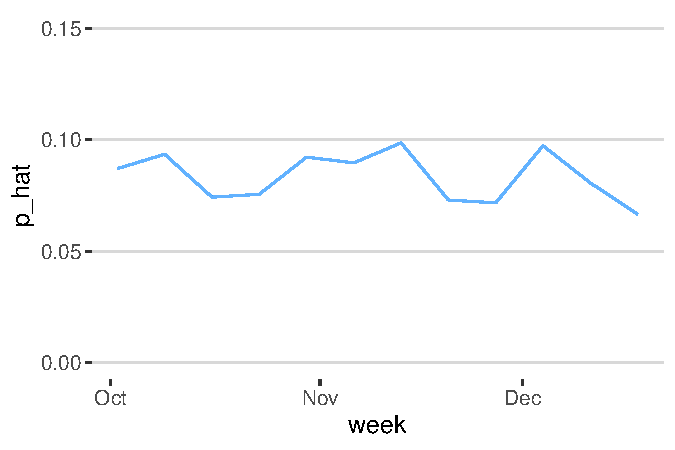
\includegraphics{HW4_files/figure-pdf/unnamed-chunk-3-1.pdf}

\subsection{\texorpdfstring{F) Calculate \(R^2\) and \(R^2_{adj}\) ``by
hand.''}{F) Calculate R\^{}2 and R\^{}2\_\{adj\} ``by hand.''}}\label{f-calculate-r2-and-r2_adj-by-hand.}

\begin{itemize}
\item
  (you can use helper functions from R to get the components needed for
  the formula, but do not simply extract it from the model object).
\item
  What do they mean?
\end{itemize}

\[
R^2=\dfrac{SS_{Reg}}{SS_Y}=1-\dfrac{RSS}{SS_Y}
\]

\[
R^2_{adj}=1-\dfrac{(1-R^2)(n-1)}{n-p}
\]

\begin{itemize}
\tightlist
\item
  Our explanatory variables crime rate, zn, and indus explain about
  \(29.4\%\) (adjusted \(r^2 = 28.9\%\)) of variation in median home
  values across suburbs.
\end{itemize}

\begin{Shaded}
\begin{Highlighting}[]
\NormalTok{broom}\SpecialCharTok{::}\FunctionTok{augment}\NormalTok{(m\_medv) }\SpecialCharTok{|\textgreater{}} \CommentTok{\# adds residuals \& predictions}
  \FunctionTok{mutate}\NormalTok{(}\AttributeTok{SS\_Y =}\NormalTok{ (medv }\SpecialCharTok{{-}} \FunctionTok{mean}\NormalTok{(medv))}\SpecialCharTok{\^{}}\DecValTok{2}\NormalTok{, }\CommentTok{\# deviations of Y}
         \AttributeTok{RSS =}\NormalTok{ .resid}\SpecialCharTok{\^{}}\DecValTok{2}\NormalTok{) }\SpecialCharTok{|\textgreater{}} \CommentTok{\# squared residuals}
  \FunctionTok{summarise}\NormalTok{(}
    
    \CommentTok{\# calculate r\_squared v}
    \AttributeTok{r\_squared =} \DecValTok{1} \SpecialCharTok{{-}}\NormalTok{ (}\FunctionTok{sum}\NormalTok{(RSS) }\SpecialCharTok{/} \FunctionTok{sum}\NormalTok{(SS\_Y)),}
    
    \CommentTok{\# adjusted r\_squared}
    \AttributeTok{adj\_r\_squared =} \DecValTok{1} \SpecialCharTok{{-}}\NormalTok{ ( }
\NormalTok{      (}\DecValTok{1} \SpecialCharTok{{-}}\NormalTok{ r\_squared) }\SpecialCharTok{*}\NormalTok{ (}\FunctionTok{n}\NormalTok{() }\SpecialCharTok{{-}} \DecValTok{1}\NormalTok{) ) }\SpecialCharTok{/}
\NormalTok{      (}\FunctionTok{n}\NormalTok{() }\SpecialCharTok{{-}} \FunctionTok{length}\NormalTok{(m\_medv}\SpecialCharTok{$}\NormalTok{coefficients)) }\CommentTok{\# sample size {-} \# of parameters}
    
\NormalTok{  )}
\end{Highlighting}
\end{Shaded}

\begin{verbatim}
# A tibble: 1 x 2
  r_squared adj_r_squared
      <dbl>         <dbl>
1     0.294         0.289
\end{verbatim}

\subsection{2. Fit a simple linear regression model with medv as a
function of zn and compare it to the model from question 1 using the
global F test and one other
method.}\label{fit-a-simple-linear-regression-model-with-medv-as-a-function-of-zn-and-compare-it-to-the-model-from-question-1-using-the-global-f-test-and-one-other-method.}

\begin{itemize}
\item
  Which model do you prefer based on the results of the comparison?
\item
  We use a General F test to examine which model to keep by testing the
  Null hypothesis that \(H_0 = RSS_{reduced} = RSS_{full}\) and we
  reject the Null hypothesis suggesting that the Residual Sum of Squares
  for the simple linear model is higher than the less parsimonious model
  with three predictors. Therefore, the more complex model minimizes the
  residuals at the expense of more predictors included in the model.
\item
  We also examine the r\_squared of the simple model, and the adjusted
  r-square of the three predictor model and find that our simple model
  leaves a lot of unexplained variability in median home values. The
  model with more predictors, (predictors = crim, zn, and indus),
  explains \(29\%\) of the variance in median home value, while the
  reduced model (predictor = zn) explains \(13\%\) of the variance in
  median home value. The adjusted R-squared adjusts for multiple
  predictors in the model, therefore, we report the adjusted
  \(adj \space R^2\) when interpreting the model with more predictor.
\item
  With a higher R-squared and lower sigma-squared (i.e variance), the
  full model is a better fit to the data and minimizes the residuals
  more so than the simple 1-predictor model.
\end{itemize}

\begin{Shaded}
\begin{Highlighting}[]
\NormalTok{m\_simple }\OtherTok{\textless{}{-}} \FunctionTok{lm}\NormalTok{(medv }\SpecialCharTok{\textasciitilde{}}\NormalTok{ zn, }\AttributeTok{data =}\NormalTok{ Boston)}

\FunctionTok{anova}\NormalTok{(m\_medv, m\_simple)}
\end{Highlighting}
\end{Shaded}

\begin{verbatim}
Analysis of Variance Table

Model 1: medv ~ crim + zn + indus
Model 2: medv ~ zn
  Res.Df   RSS Df Sum of Sq      F    Pr(>F)    
1    502 30170                                  
2    504 37167 -2   -6996.6 58.209 < 2.2e-16 ***
---
Signif. codes:  0 '***' 0.001 '**' 0.01 '*' 0.05 '.' 0.1 ' ' 1
\end{verbatim}

\begin{Shaded}
\begin{Highlighting}[]
\FunctionTok{message}\NormalTok{(}
  \FunctionTok{str\_c}\NormalTok{(}\FunctionTok{cat}\NormalTok{(}
    \StringTok{"The R{-}squared for the simple model is "}\NormalTok{, }
        \FunctionTok{round}\NormalTok{(}\FunctionTok{summary}\NormalTok{(m\_simple)}\SpecialCharTok{$}\NormalTok{r.squared, }\DecValTok{3}\NormalTok{), }
        \StringTok{" (adjusted R{-}squared "}\NormalTok{, }
        \FunctionTok{round}\NormalTok{(}\FunctionTok{summary}\NormalTok{(m\_simple)}\SpecialCharTok{$}\NormalTok{r.squared, }\DecValTok{3}\NormalTok{), }\StringTok{").}\SpecialCharTok{\textbackslash{}n}\StringTok{"}
\NormalTok{    ), }
        \FunctionTok{cat}\NormalTok{(}
          \StringTok{" The adjusted R{-}squared for the model with 3 predictors is "}\NormalTok{,}
        \FunctionTok{round}\NormalTok{(}\FunctionTok{summary}\NormalTok{(m\_medv)}\SpecialCharTok{$}\NormalTok{adj.r.squared, }\DecValTok{3}\NormalTok{) }
\NormalTok{        )}
\NormalTok{    )}
\NormalTok{)}
\end{Highlighting}
\end{Shaded}

\begin{verbatim}
The R-squared for the simple model is  0.13  (adjusted R-squared  0.13 ).
 The adjusted R-squared for the model with 3 predictors is  0.289
\end{verbatim}

\begin{verbatim}
\end{verbatim}



\end{document}
